\documentclass[xetex,mathsans,sans,aspectratio=169]{beamer}
\usetheme{Boadilla}
\usecolortheme{orchid}
\usepackage{fontspec}
\setsansfont{Basis Grotesque}
\setbeamertemplate{navigation symbols}{}


\title[NuCypher]{
\includegraphics[width=5.5cm]{pdf/nucypher_logo.pdf}}
\author[<fname>]{<fname lname>, <title>}
\date[<dd Mon yyyy>]{<event>, <dd Mon yyyy>}

\begin{document}
    \begin{frame}
        \titlepage
    \end{frame}

    \begin{frame}
      \frametitle{Problem}
      \framesubtitle{Data Breaches}
        \begin{figure}
            \centering
            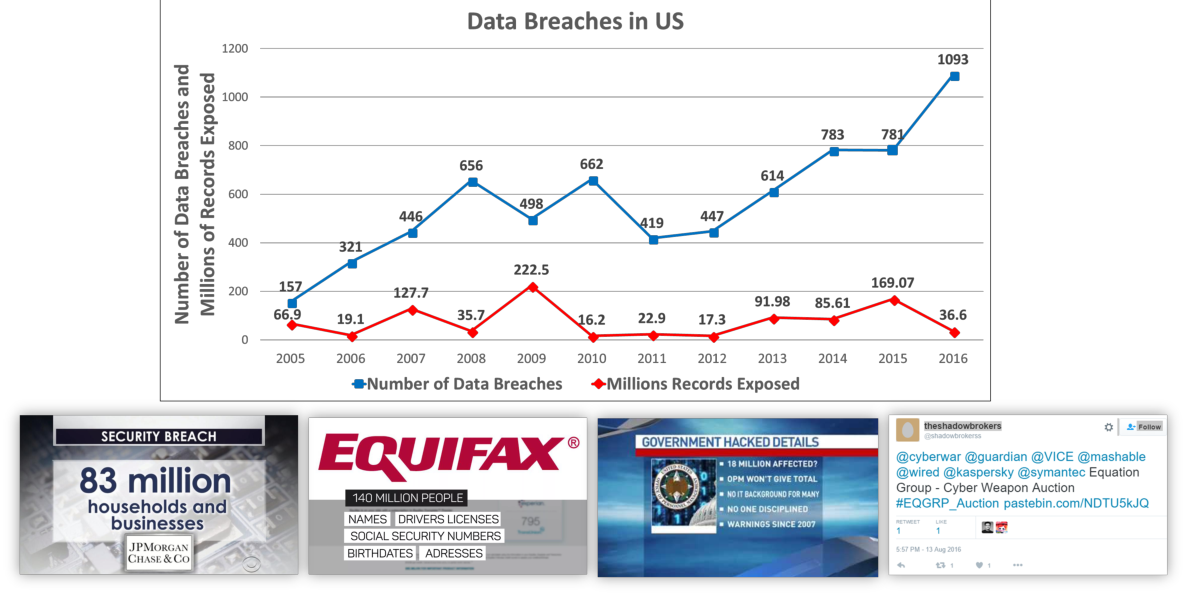
\includegraphics[height=6cm]{pdf/data-breaches.pdf}
        \end{figure}

        {\tiny Source: \url{https://www.statista.com/statistics/273550/data-breaches-recorded-in-the-united-states-by-number-of-breaches-and-records-exposed/} \par}
    \end{frame}

    \begin{frame}
      \frametitle{Impact of Data Breaches}
        \begin{figure}
            \centering
            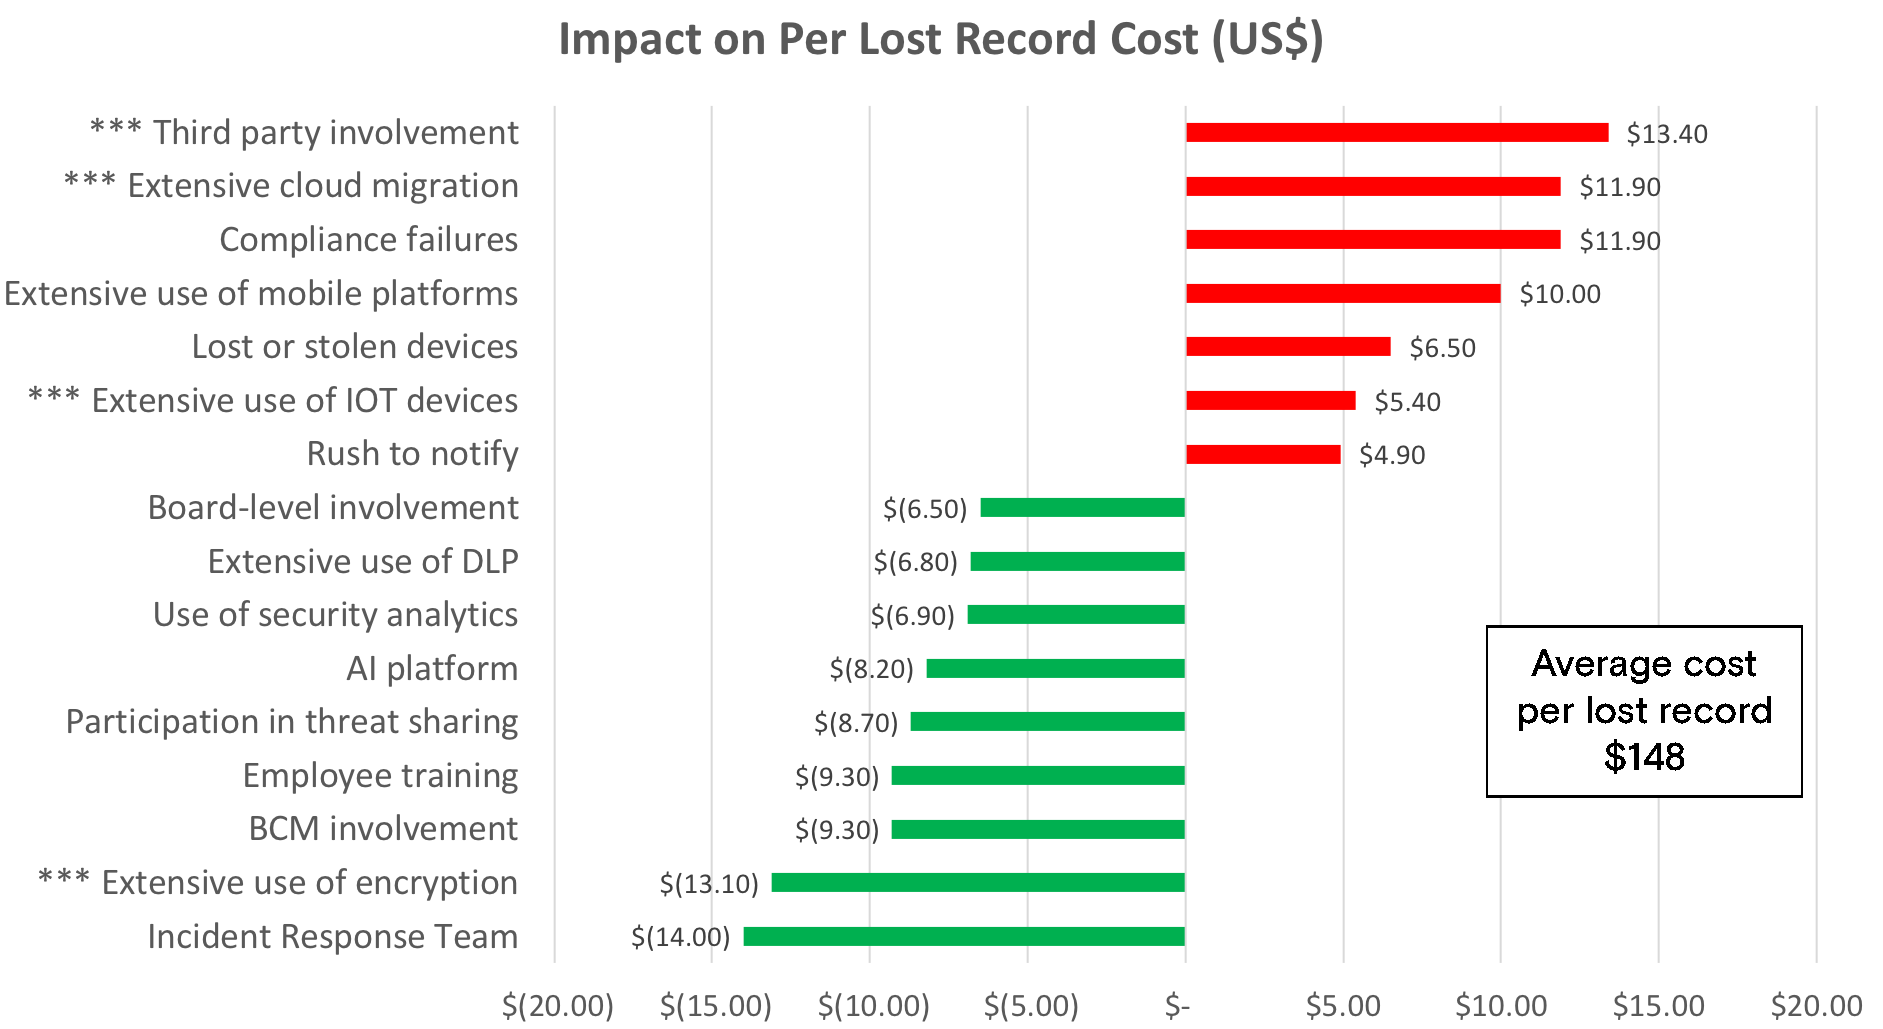
\includegraphics[height=6.5cm]{pdf/impact-of-data-breaches.pdf}
        \end{figure}

        {\tiny Source: IBM 2018 Cost of a Data Breach Study: Global Overview, \url{https://www.ibm.com/security/data-breach} \par}
    \end{frame}

    \begin{frame}
        \frametitle{Public Key Encryption (PKE)}
        \begin{figure}
            \centering
            \includegraphics<1>[width=11cm]{pdf/pke-multi.pdf}
            \includegraphics<2>[width=11cm]{pdf/pke-multi-hack.pdf}
        \end{figure}

        Limitations
        \begin{itemize}
            \item Decryption required before sharing
            \item Not scalable
            \item Complex access revocation
        \end{itemize}
    \end{frame}

    \begin{frame}
        \frametitle{What is proxy re-encryption (PRE)}
        \begin{figure}
            \centering
            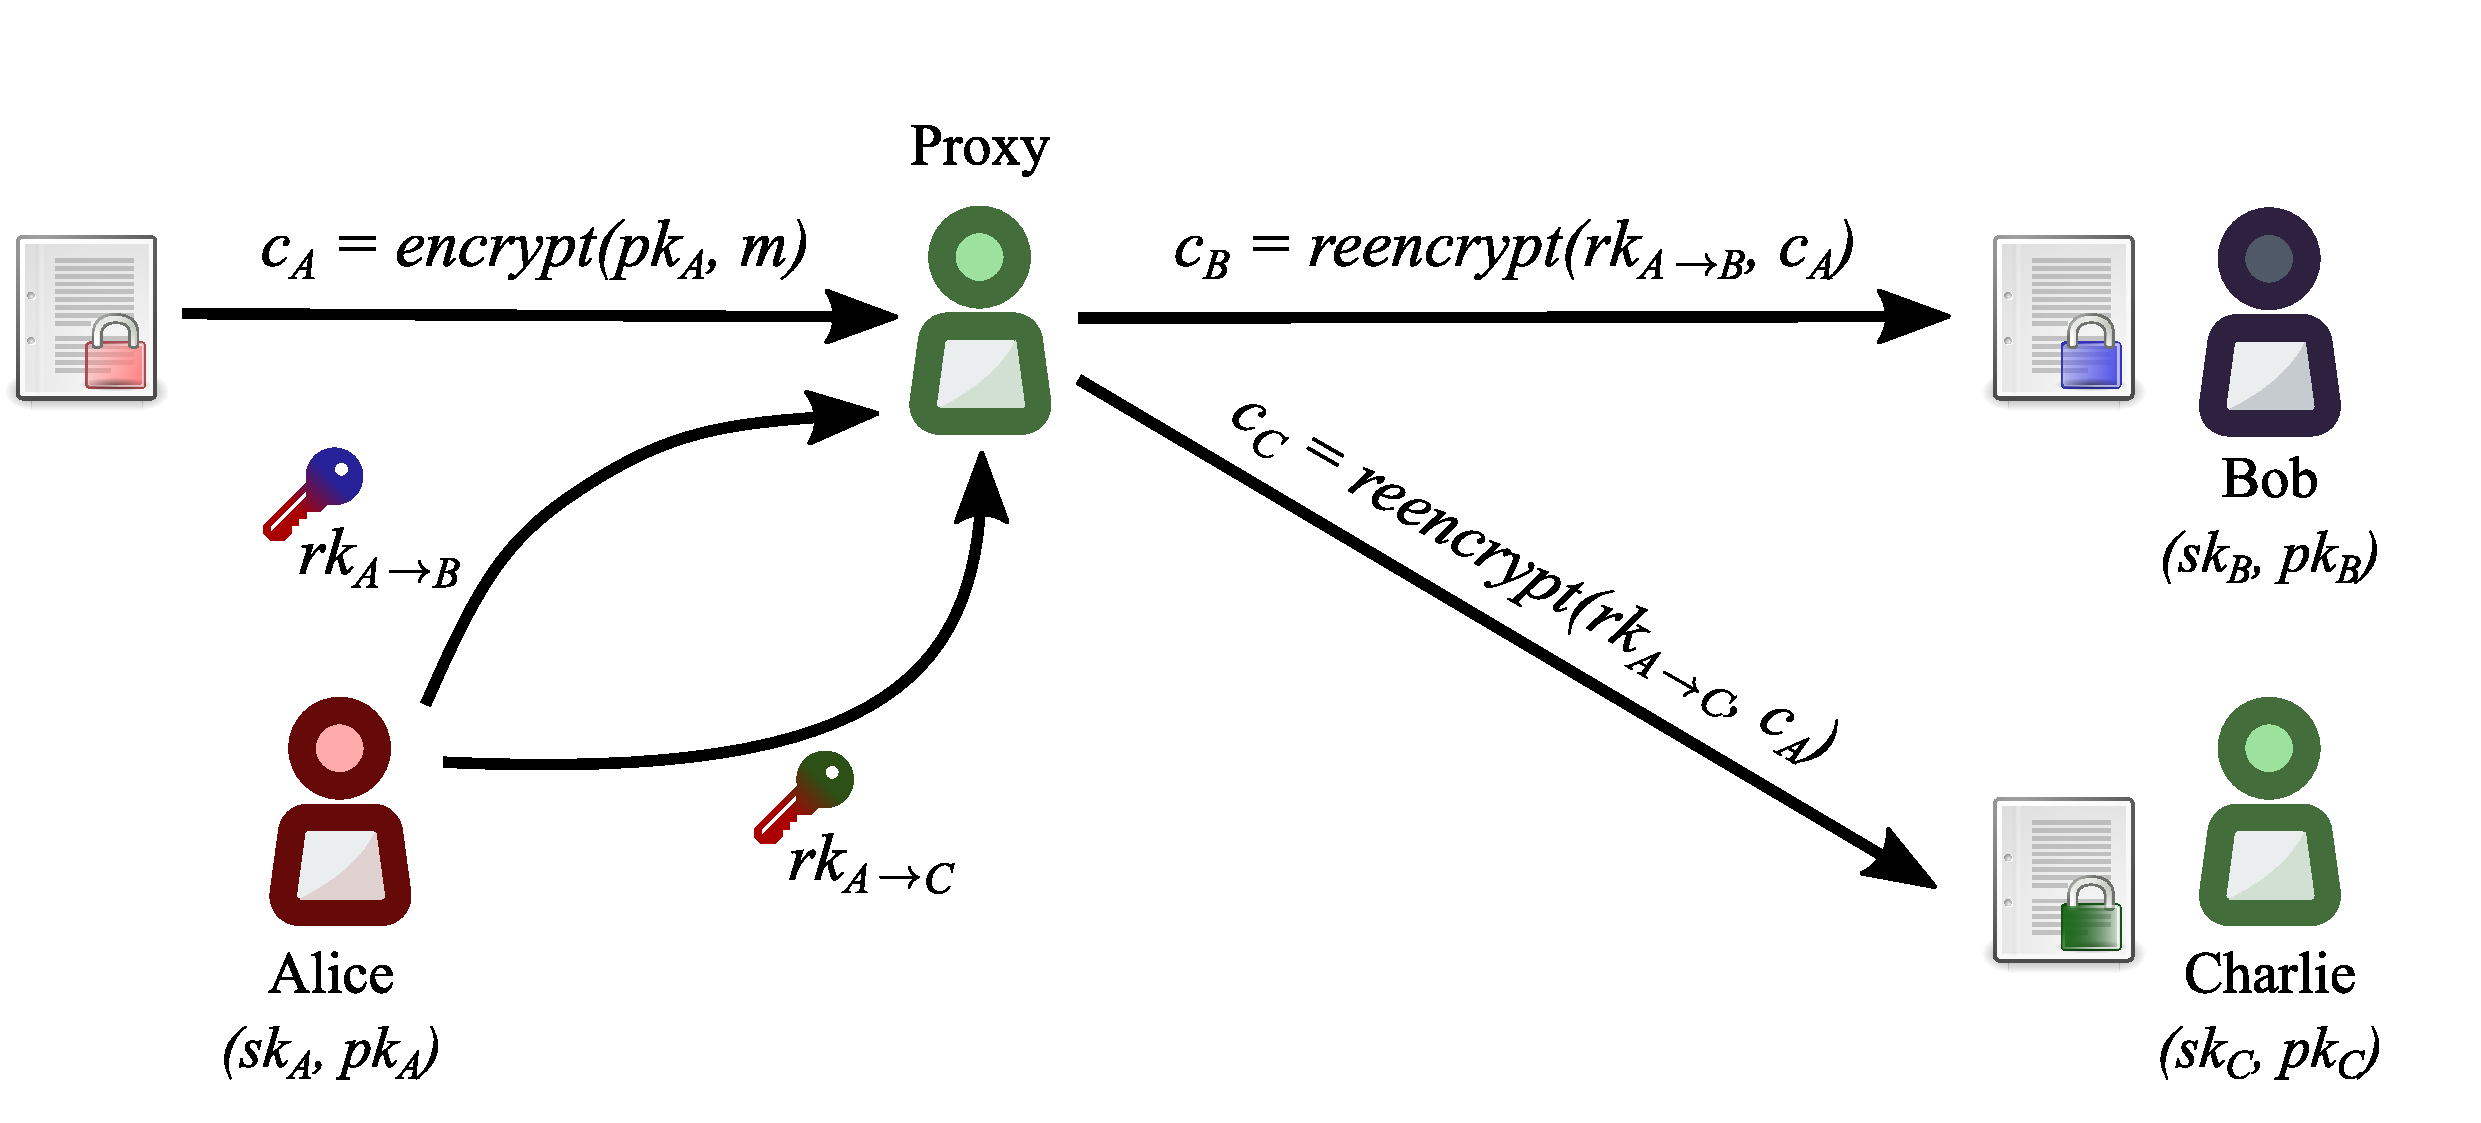
\includegraphics[width=11cm]{pdf/pre-multi.pdf}
        \end{figure}
    \end{frame}

    \begin{frame}
        \frametitle{Solution}
        \framesubtitle{Proxy Re-encryption + KMS}
        \begin{figure}
            \centering
            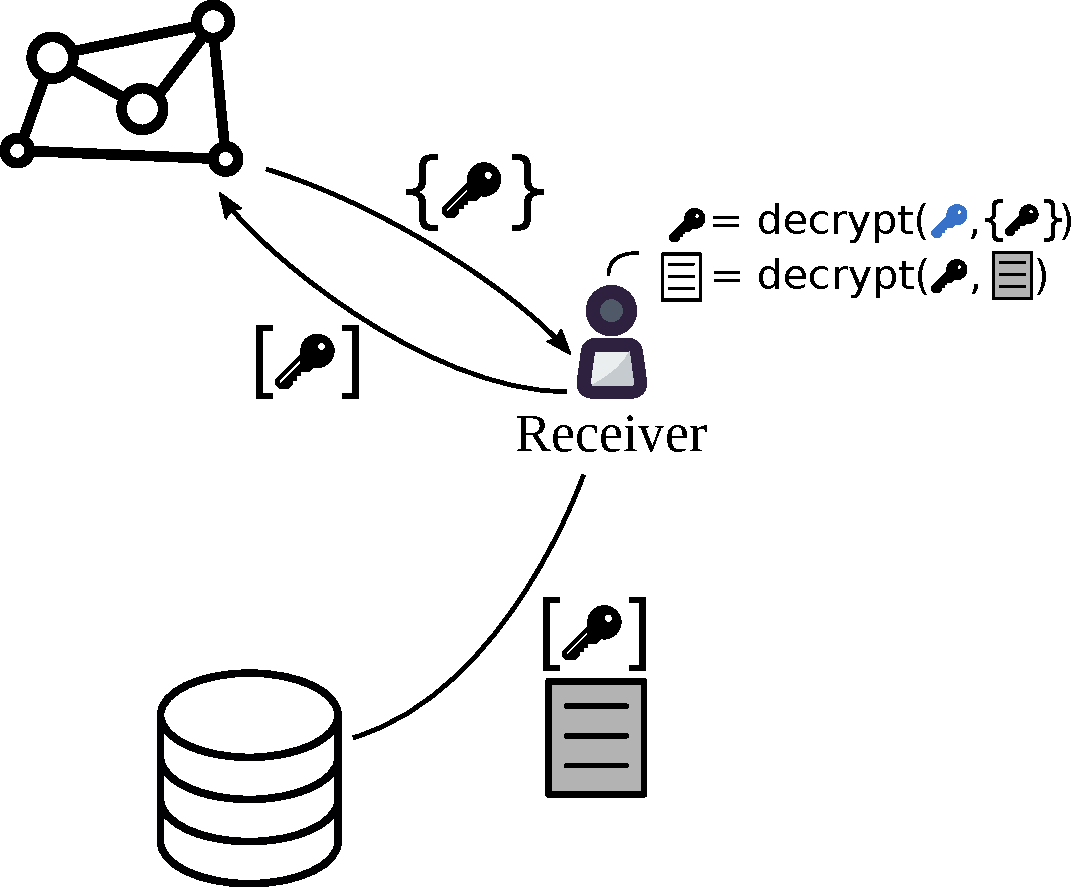
\includegraphics[height=5cm]{pdf/pre-kms.pdf}
        \end{figure}

        Advantages
        \begin{itemize}
            \item Data not decrypted to facilitate sharing
            \item Scalable and performant
            \item Access revocation through re-encryption key deletion
            \item Secure use of data storage providers
        \end{itemize}
    \end{frame}

    \begin{frame}
        \frametitle{Centralized KMS using PRE}
        \framesubtitle{Encryption}
        \begin{figure}
            \centering
            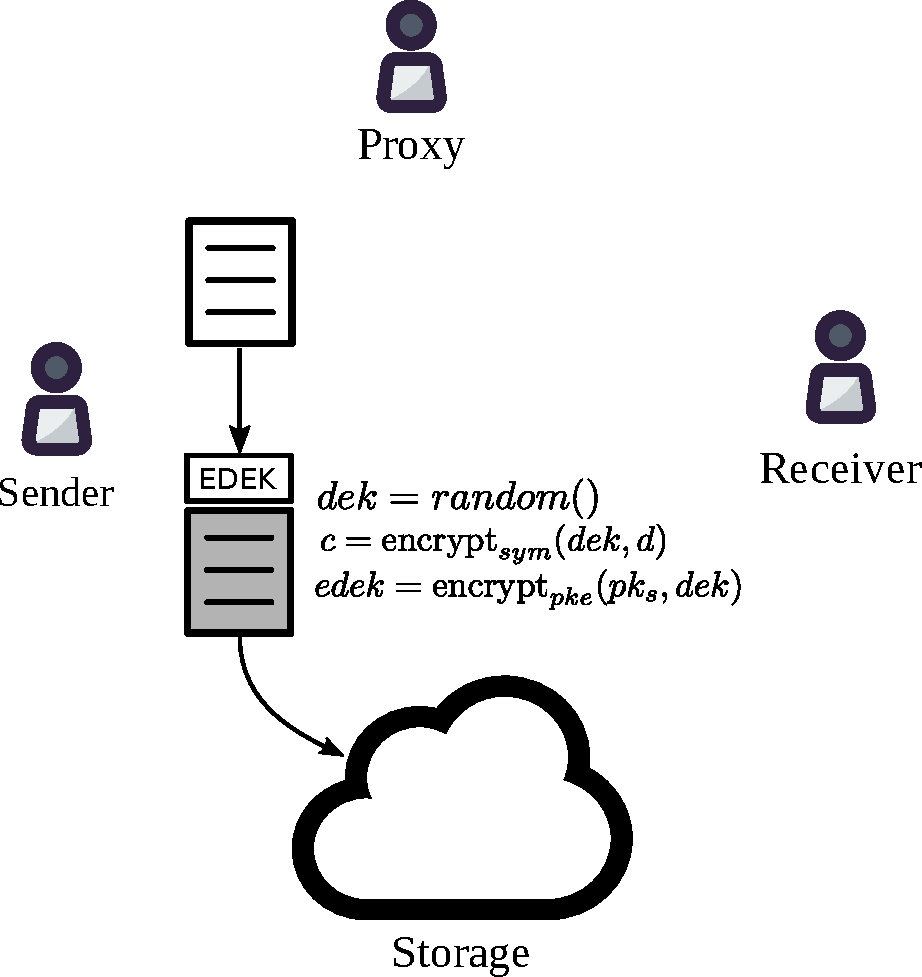
\includegraphics[height=5.5cm]{pdf/encrypt.pdf}
        \end{figure}
    \end{frame}

    \begin{frame}
        \frametitle{Centralized KMS using PRE}
        \framesubtitle{Access delegation}
        \begin{figure}
            \centering
            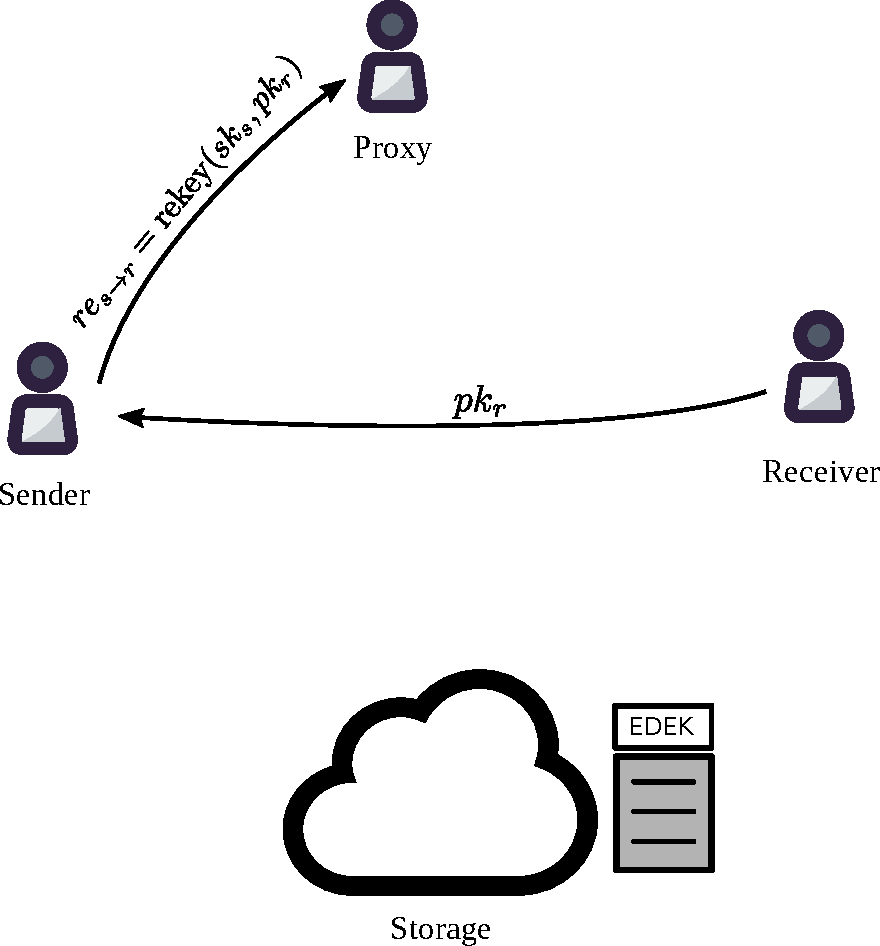
\includegraphics[height=5.5cm]{pdf/delegate.pdf}
        \end{figure}
    \end{frame}

    \begin{frame}
        \frametitle{Centralized KMS using PRE}
        \framesubtitle{Decryption}
        \begin{figure}
            \centering
            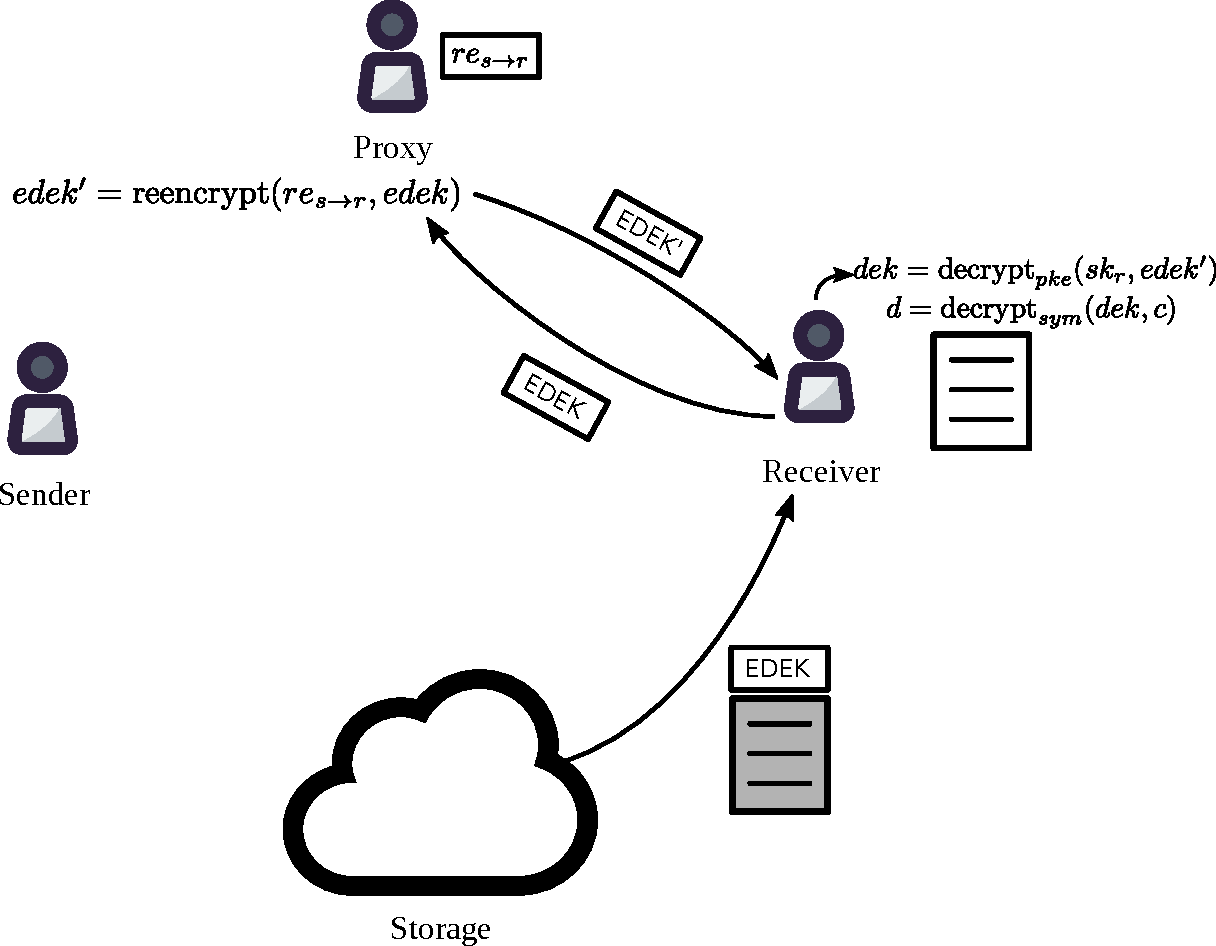
\includegraphics[height=5.5cm]{pdf/decrypt.pdf}
        \end{figure}
    \end{frame}

    \begin{frame}
        \frametitle{Decentralized KMS using PRE}
        \framesubtitle{Using threshold split-key re-encryption (Umbral)}
        \begin{figure}
            \centering
            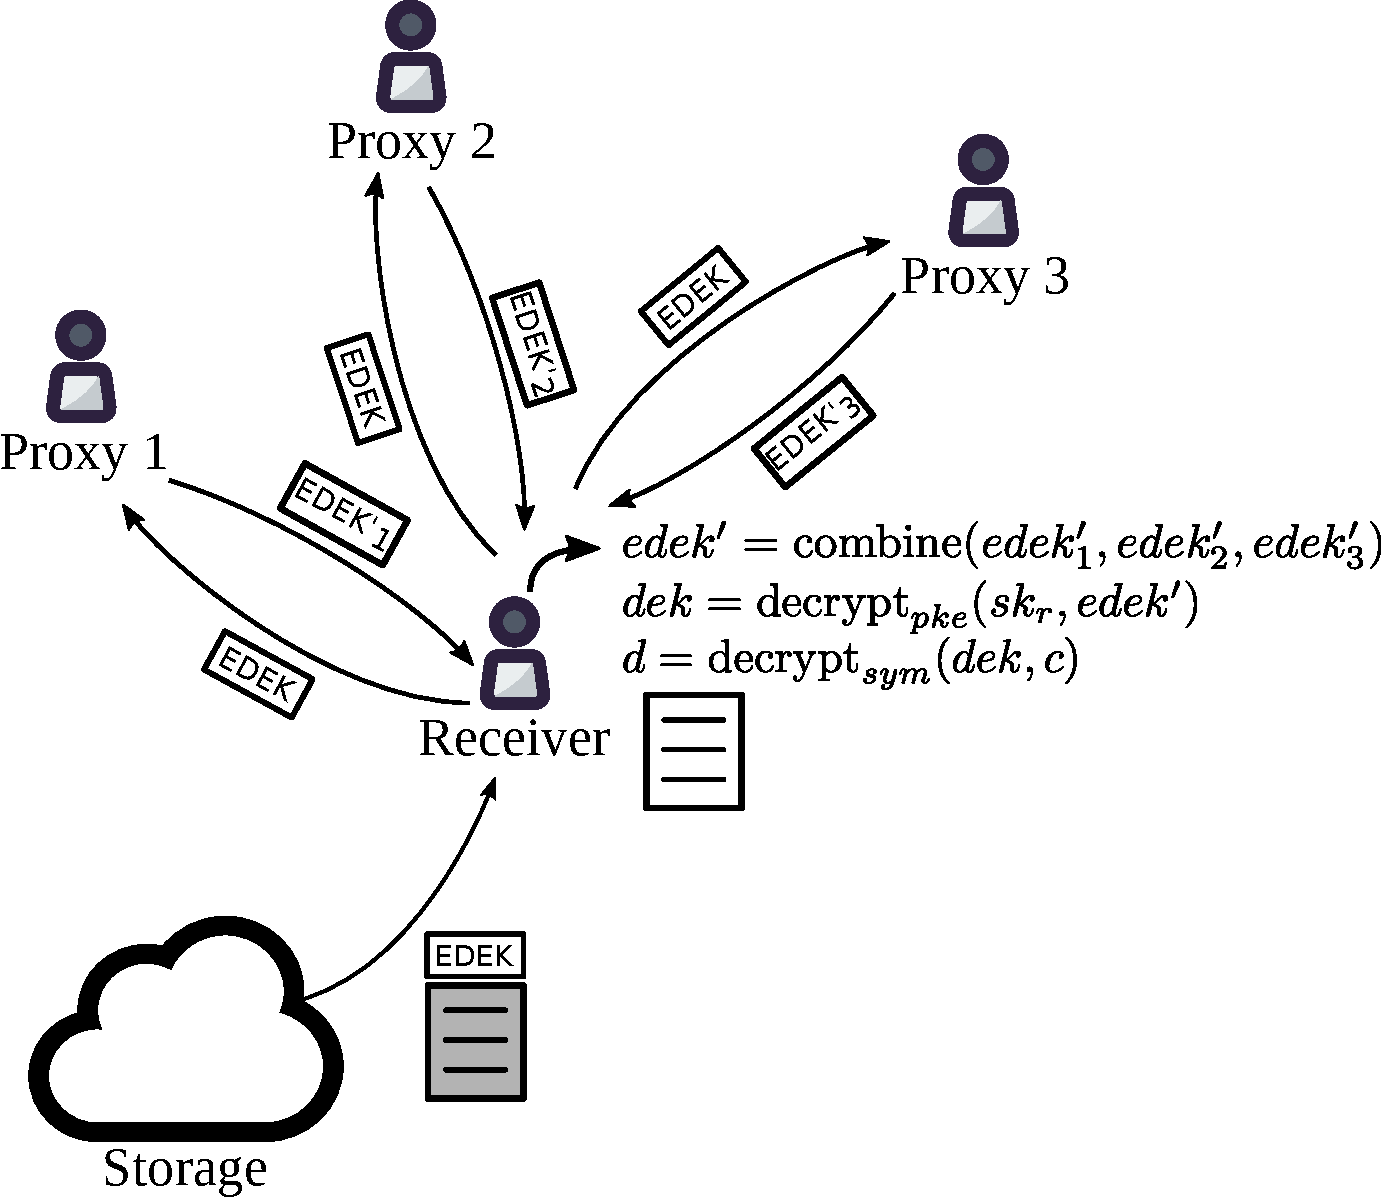
\includegraphics[height=6.5cm]{pdf/decrypt-umbral.pdf}
        \end{figure}
    \end{frame}

    \begin{frame}
        \frametitle{Decentralized KMS: Token}
        \framesubtitle{Purpose}
        \begin{itemize}
            \item Splitting trust between re-encryption nodes (more tokens = more trust and more work)
            \item Proof of Stake for minting new coins according to the mining schedule
            \item Security deposit to be at stake against malicious behavior of nodes
        \end{itemize}
    \end{frame}

    \begin{frame}
        \frametitle{Blockchain \& Smart Contract Agnostic}
        \begin{figure}
            \centering
            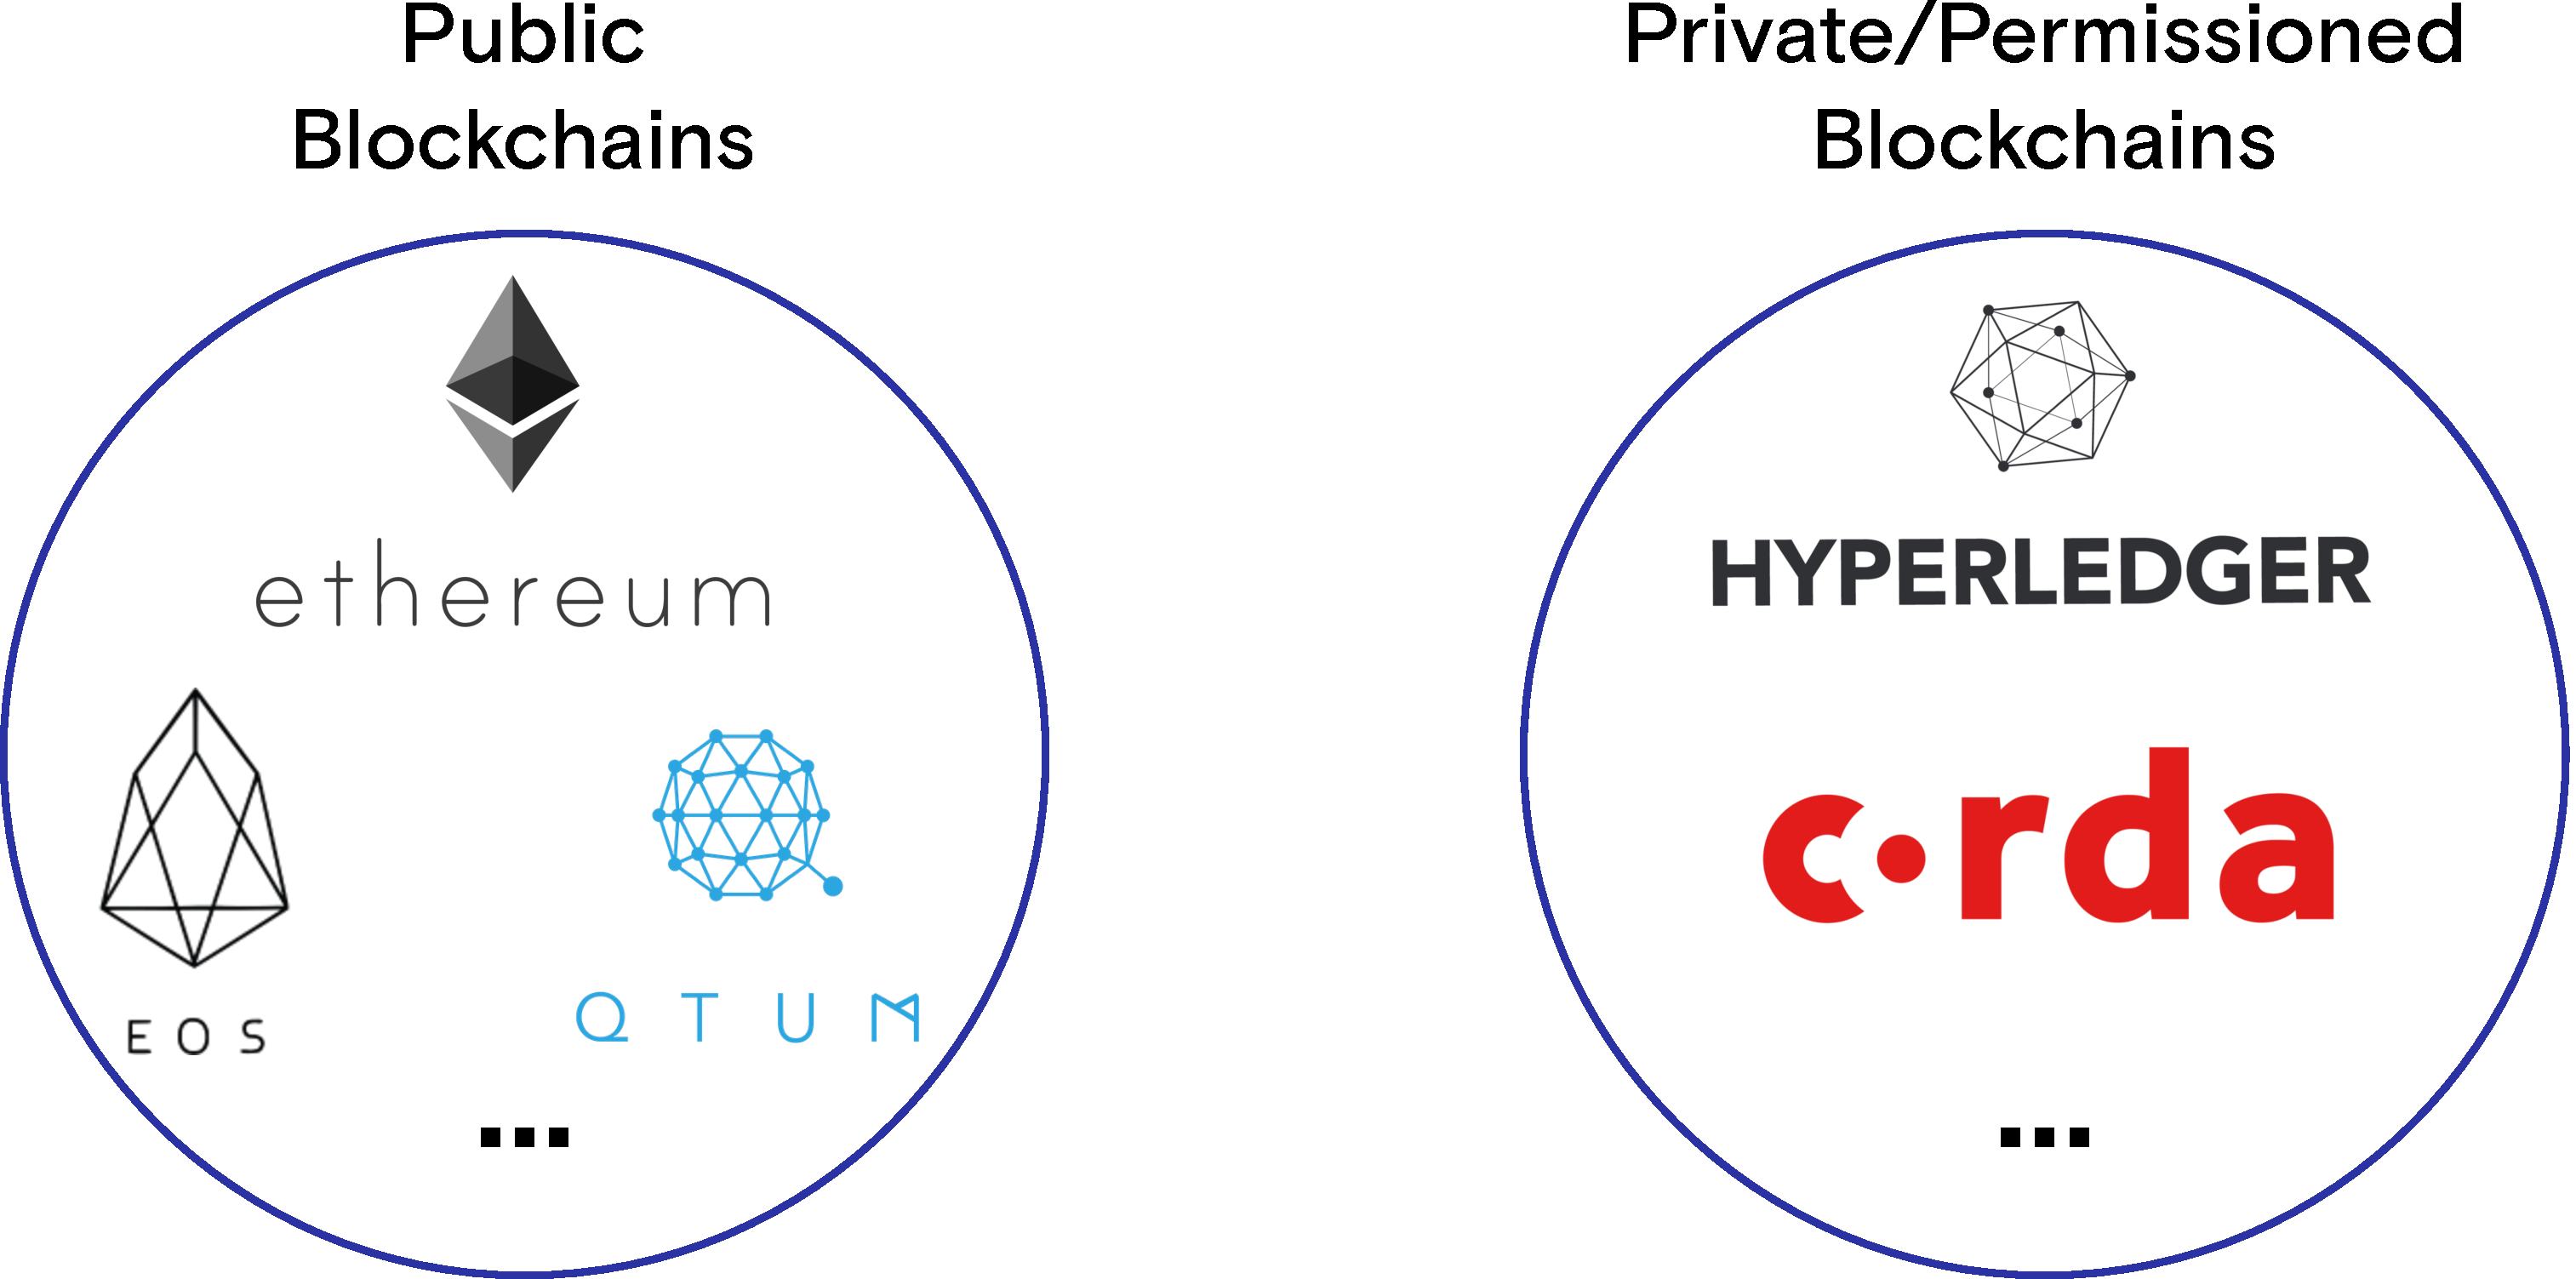
\includegraphics[height=6cm]{pdf/blockchains.pdf}
        \end{figure}
    \end{frame}

    \begin{frame}
        \frametitle{Use Cases}
        \framesubtitle{Multi-tenant, Multi-source Encrypted Data Lake}
        \begin{figure}
            \centering
            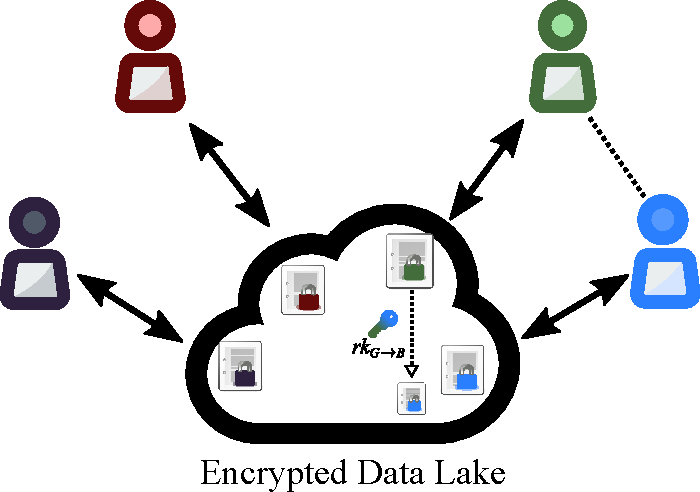
\includegraphics[height=7.5cm]{pdf/data-lake.pdf}
        \end{figure}
    \end{frame}

    \begin{frame}
        \frametitle{Use Cases}
        \framesubtitle{Scalable, Secure IOT Updates}
        \begin{figure}
            \centering
            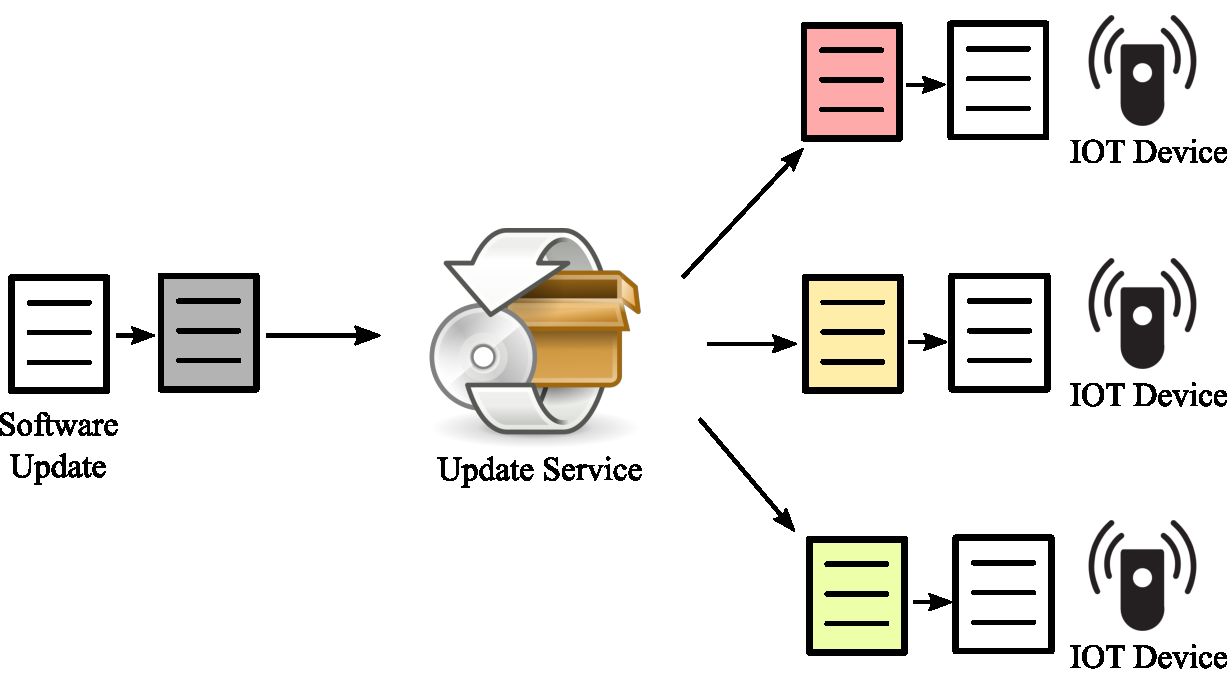
\includegraphics[height=6cm]{pdf/iot-updates.pdf}
        \end{figure}
    \end{frame}

    \begin{frame}
        \frametitle{Use Cases}
        \framesubtitle{Encrypted file sharing}
        \begin{figure}
            \centering
            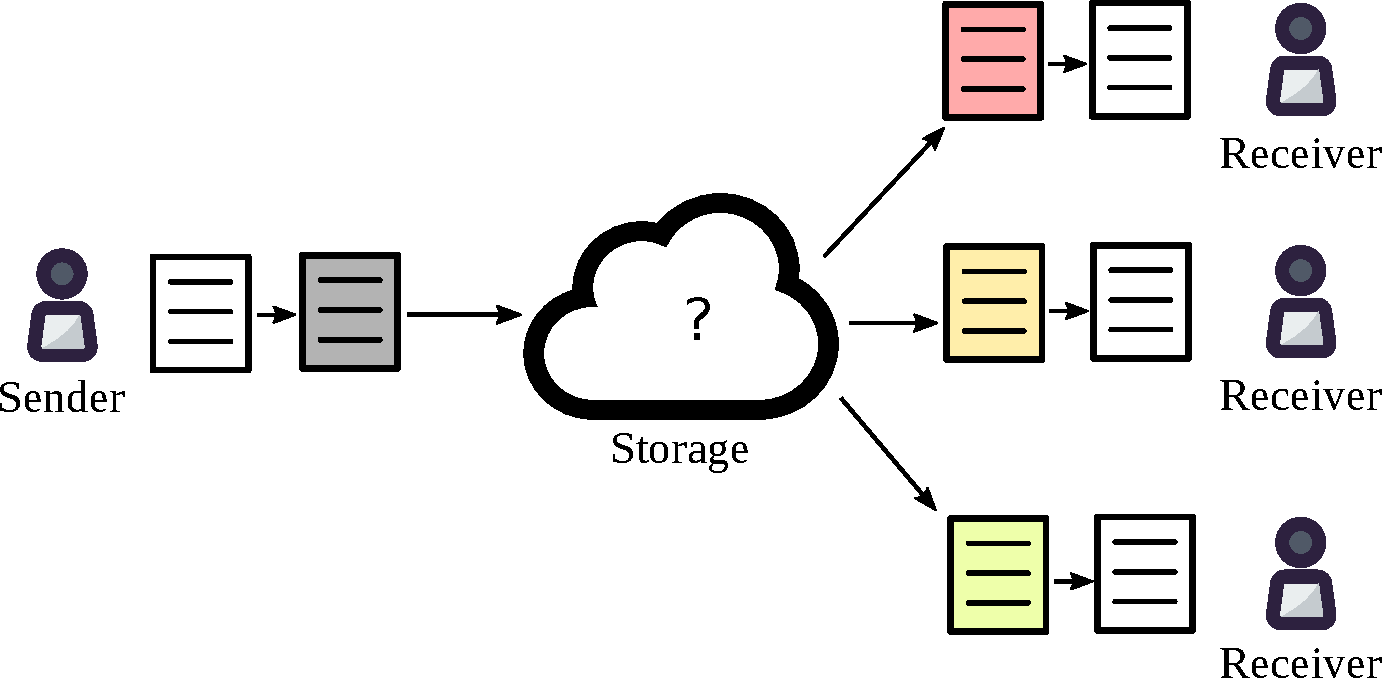
\includegraphics[height=5.5cm]{pdf/file-sharing.pdf}
        \end{figure}
    \end{frame}

    \begin{frame}
        \frametitle{Use Cases}
        \framesubtitle{Encrypted multi-user chats}
        \begin{figure}
            \centering
            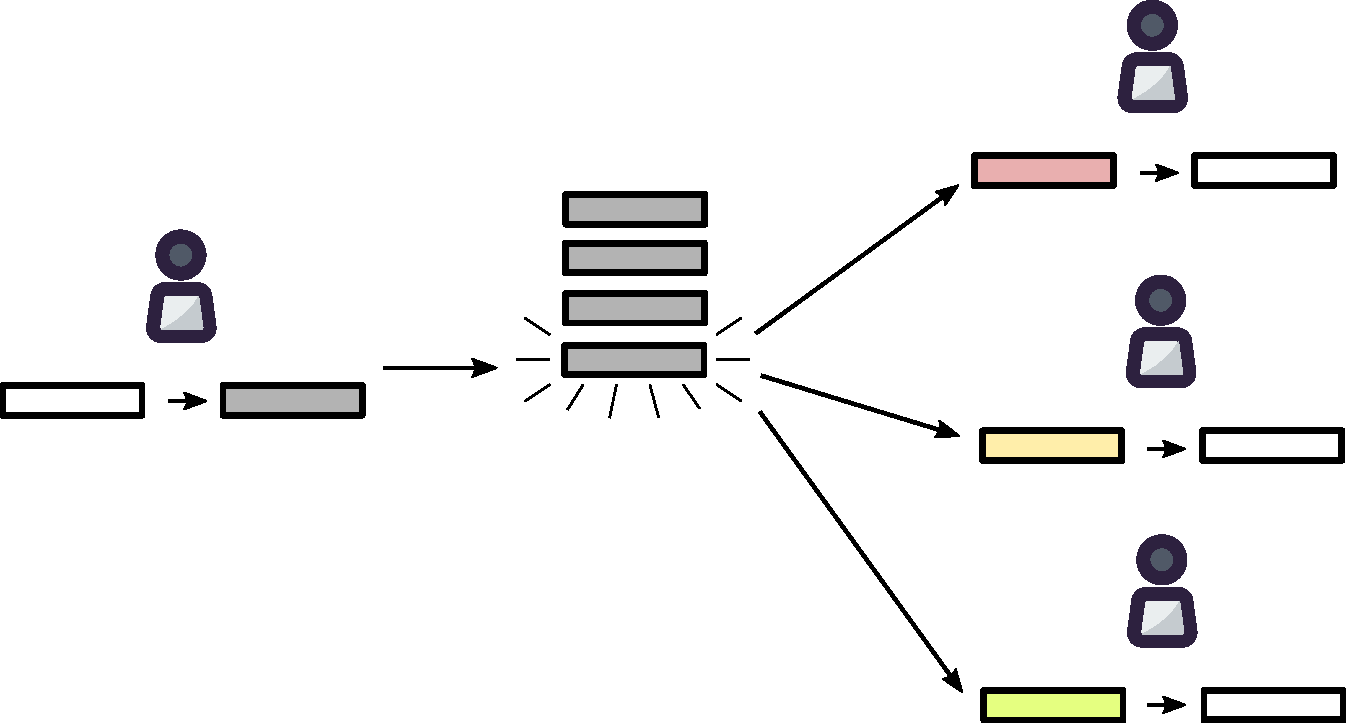
\includegraphics[height=5cm]{pdf/chats.pdf}
        \end{figure}
    \end{frame}

    \begin{frame}
        \frametitle{Use Cases}
        \framesubtitle{Decentralized Access-Controlled Content}
        \begin{figure}
            \centering
            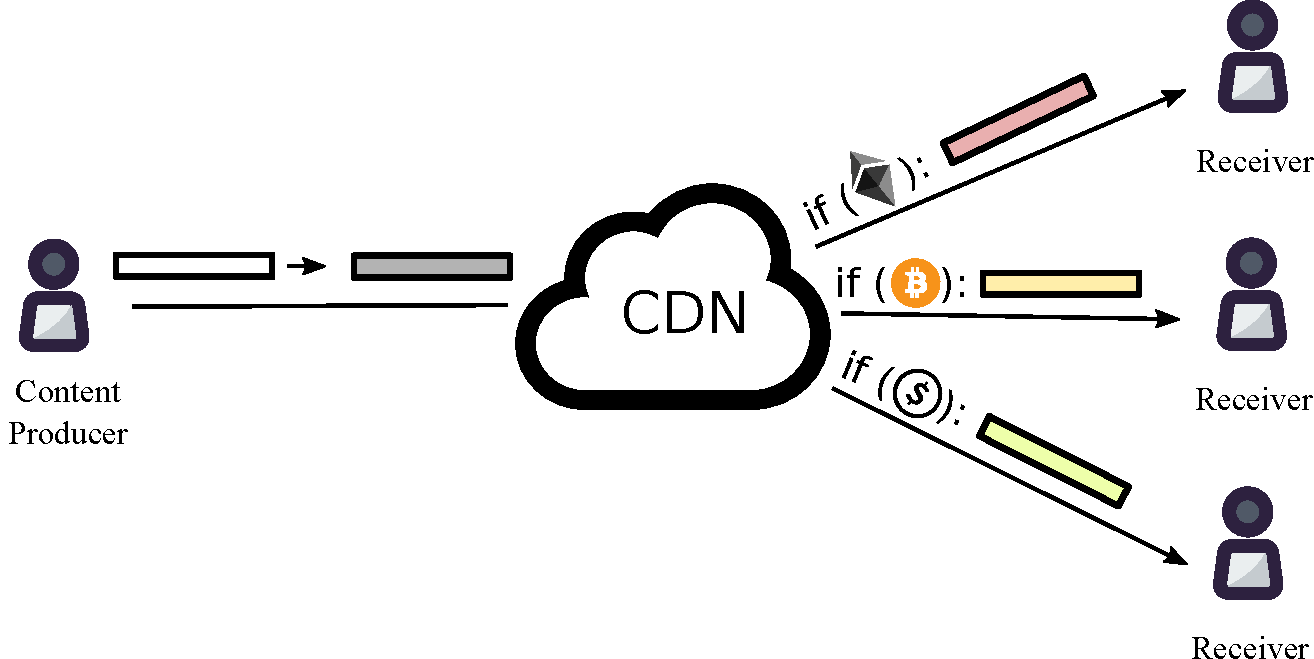
\includegraphics[height=5.5cm]{pdf/content.pdf}
        \end{figure}
    \end{frame}

    \begin{frame}
      \frametitle{Early Users}
      \begin{figure}
           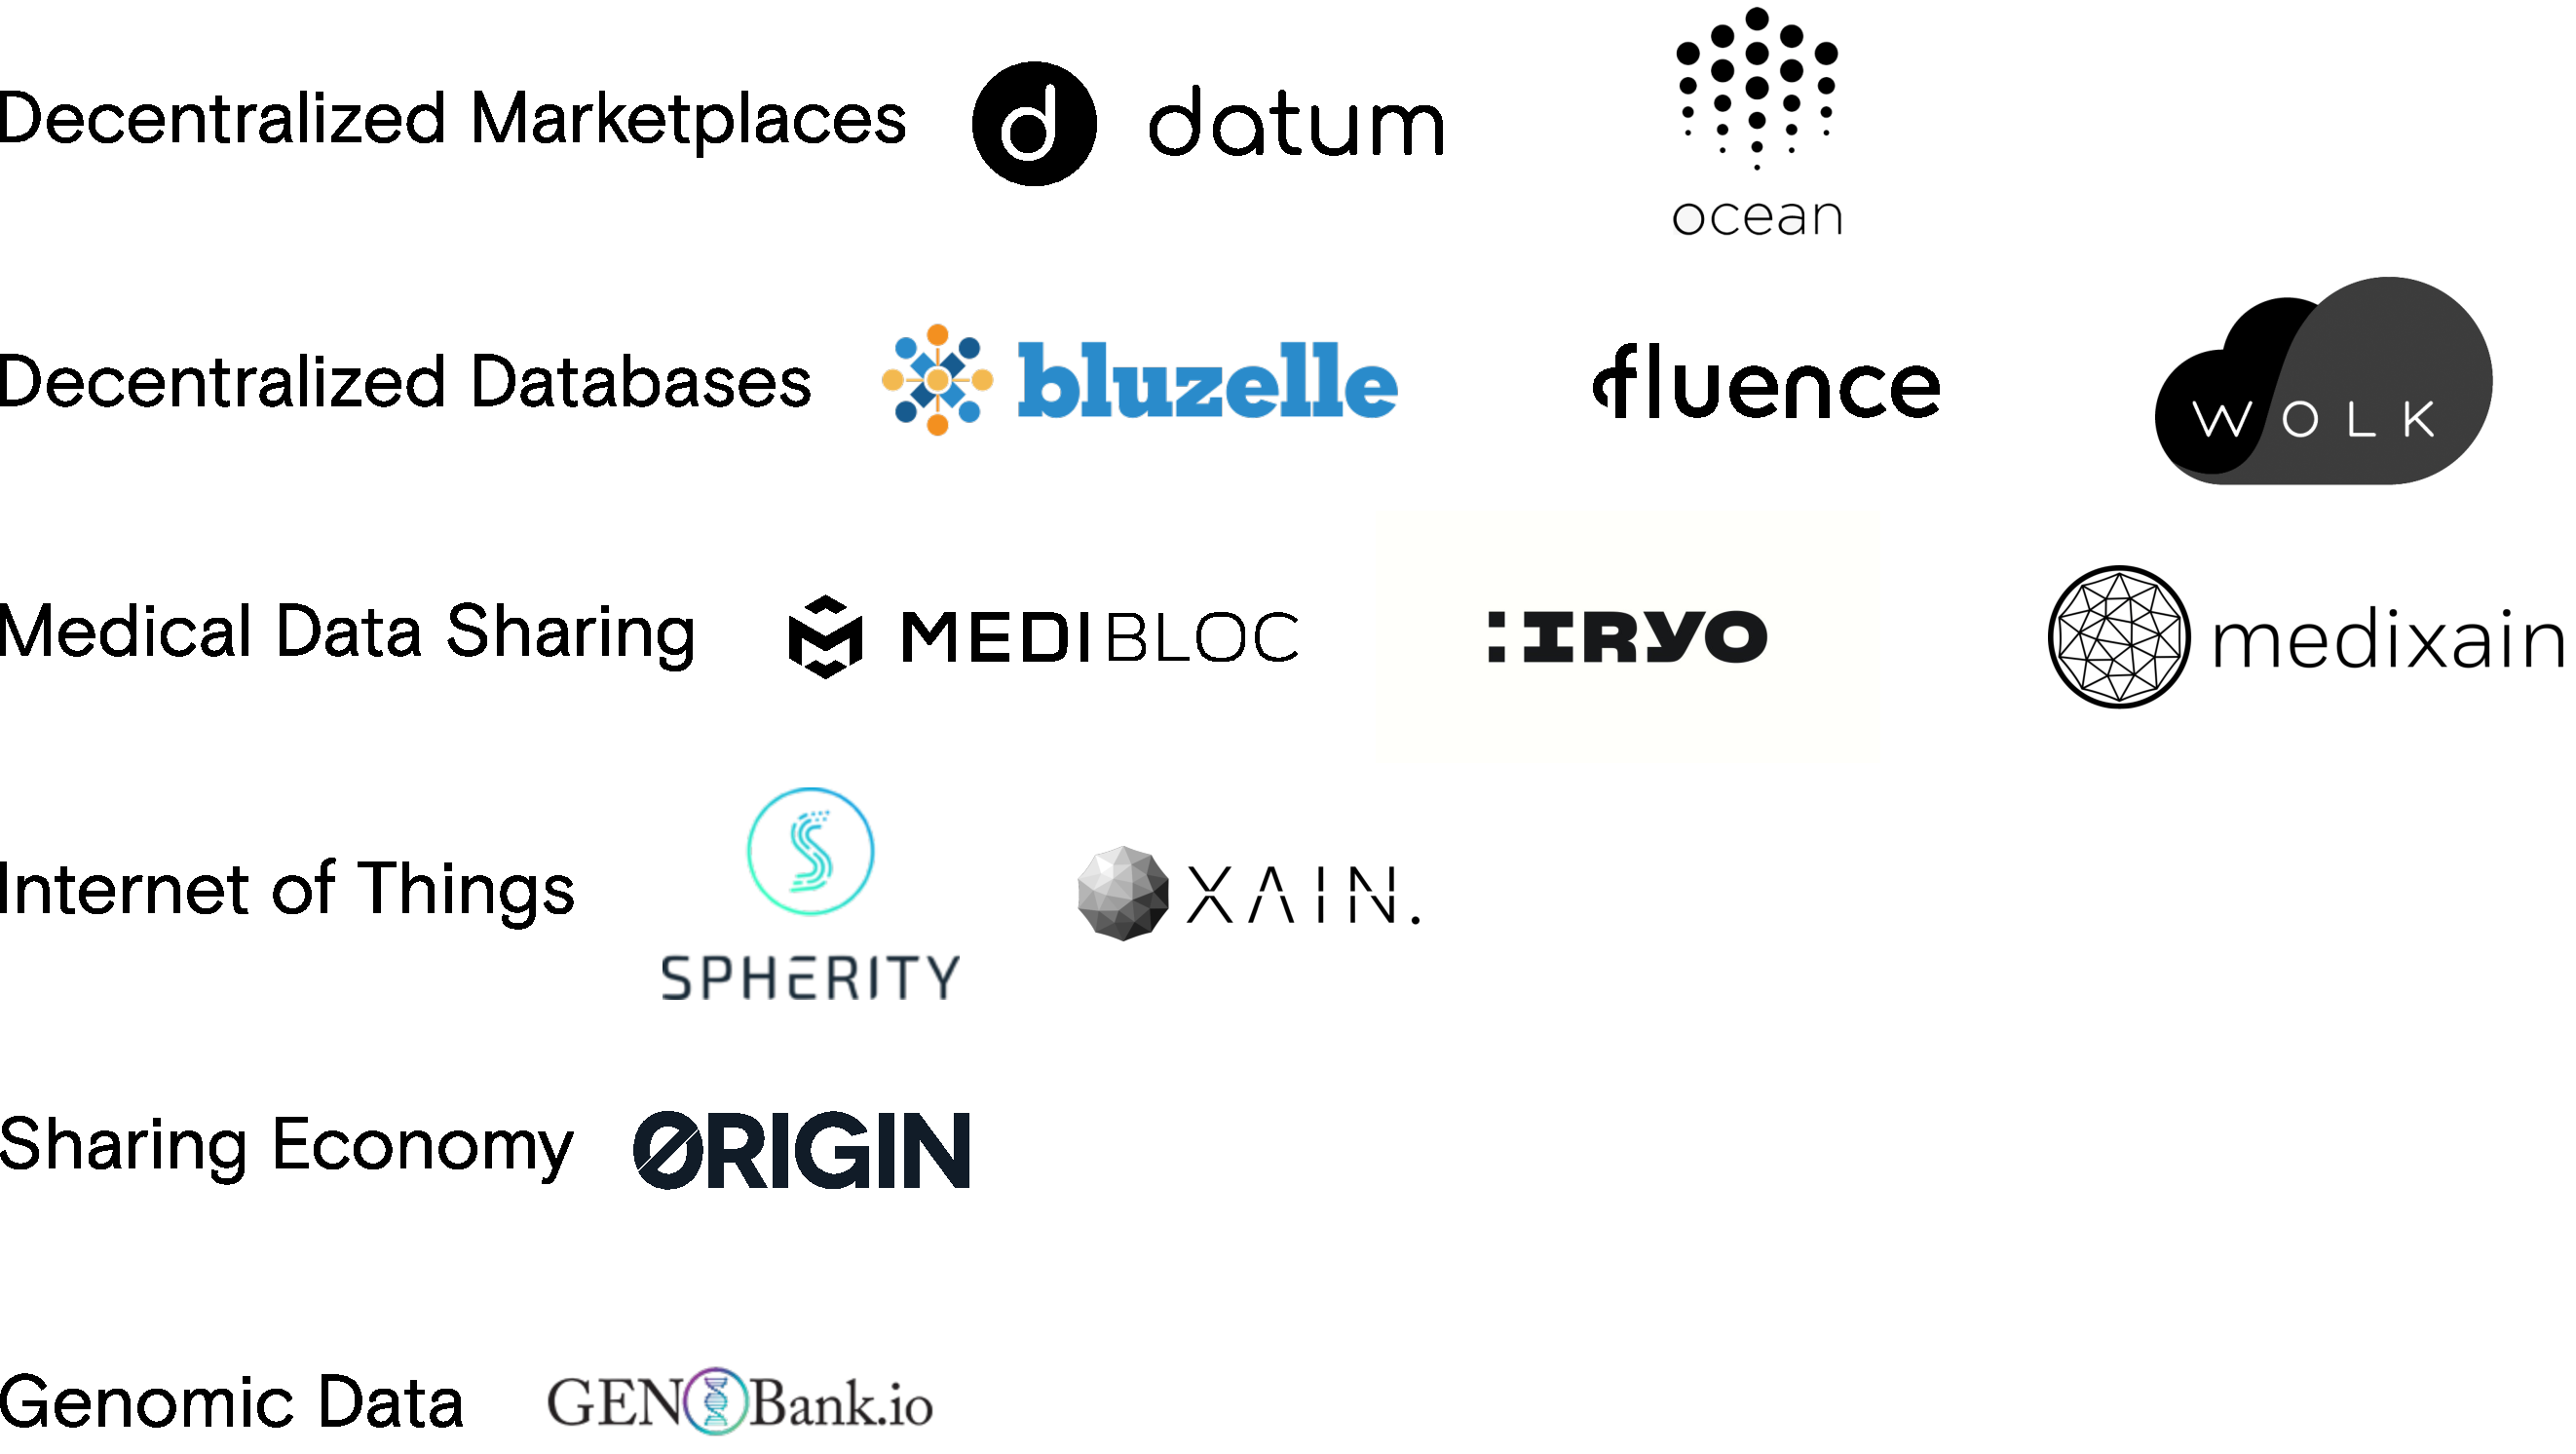
\includegraphics[width=11.5cm]{pdf/projects.pdf}
      \end{figure}
    \end{frame}

    \begin{frame}
      \frametitle{Competing Technology}
       Data Masking and Tokenization
       \begin{itemize}
           \item Less secure for data with underlying patterns
           \item Reduce the value of data by obfuscating it
       \end{itemize}

       Multi-Party Computation
       \begin{itemize}
           \item Early Research Stage
           \item Slow Performance
       \end{itemize}
      
       Fully Homomorphic Encryption
       \begin{itemize}
           \item Early Research Stage
           \item Slow Peformance
           \begin{itemize}
               \item \emph{NuCypher has invested efforts in this area}
           \end{itemize}
       \end{itemize}
       
     \end{frame}
    
    \begin{frame}
      \frametitle{Investors}
        \framesubtitle{>\$15M in Venture Funding}
        \begin{figure}
            \centering
            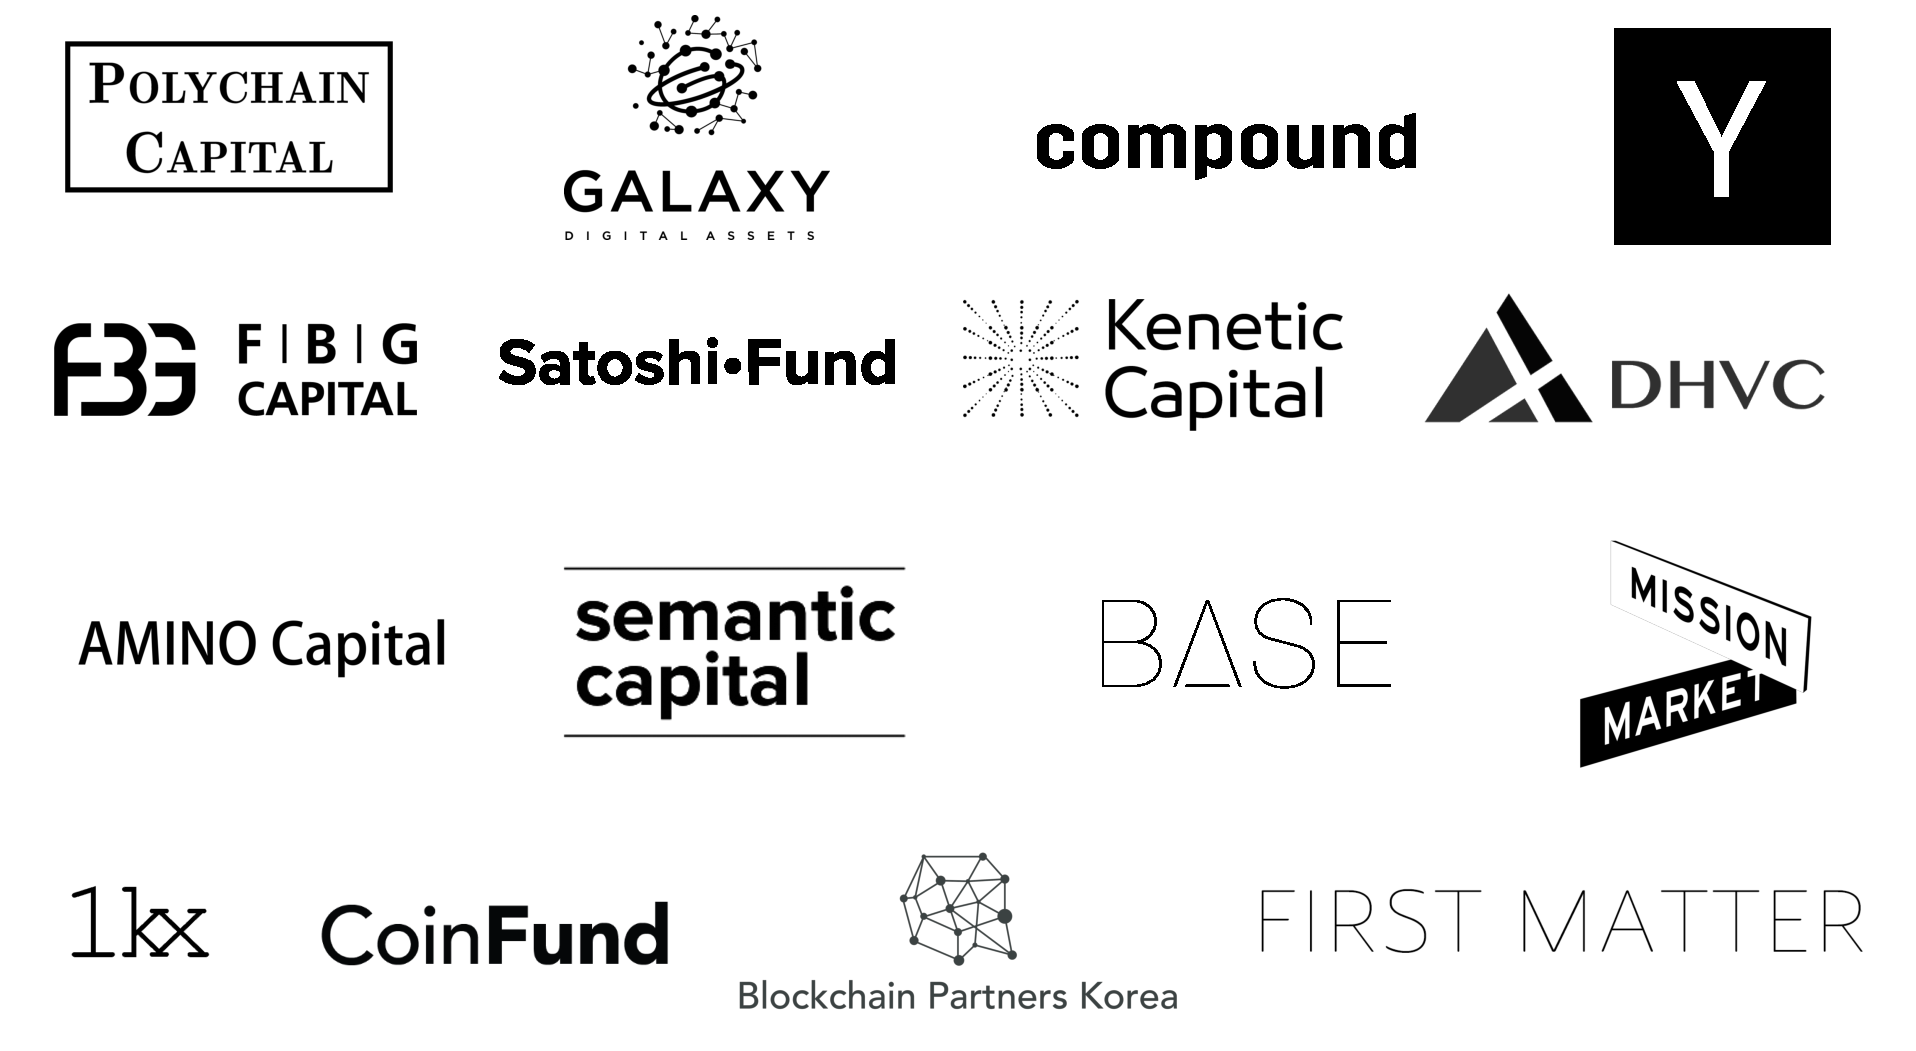
\includegraphics[height=6.5cm]{pdf/investors.pdf}
        \end{figure}
    \end{frame}

    \begin{frame}
      \frametitle{Team}
        \begin{figure}
            \centering
            \includegraphics[width=15cm]{pdf/company.pdf}
        \end{figure}
    \end{frame}

    \begin{frame}
        \frametitle{More Information}
        \begin{figure}
            \centering
            
\includegraphics[width=5cm]{pdf/nucypher_logo.pdf}
        \end{figure}
        Website: \url{https://nucypher.com}

        Whitepaper: \url{https://www.nucypher.com/whitepapers/english.pdf}

        Github: \url{https://github.com/nucypher}

        Discord: \url{https://discord.gg/7rmXa3S}

        Email: \href{mailto:<fname>@nucypher.com}{<fname>@nucypher.com}

        Email: \href{mailto:hello@nucypher.com}{hello@nucypher.com}
    \end{frame}

    \begin{frame}
      \frametitle{Appendix: Umbral - Threshold Proxy Re-Encryption}
      Designed by: David Nu\~{n}ez, University of Malaga, NICS Lab
      \begin{itemize}
          \item \emph{``Umbral''} is Spanish for \emph{``threshold''}
          \item PRE properties: Unidirectional, single-hop, non-interactive
          \item It follows a KEM/DEM approach:
          \begin{itemize}
              \item UmbralKEM provides the threshold re-encryption capability
              \item The DEM can be any authenticated encryption (currently ChaCha20-Poly1305)
          \end{itemize}
          \item IND-PRE-CCA security
          \item Verification of re-encryption correctness through Non-Interactive ZK Proofs
          \item Code: \url{https://github.com/nucypher/pyUmbral/}
          \item Documentation (WIP): \url{https://github.com/nucypher/umbral-doc}
      \end{itemize}
    \end{frame}

    \begin{frame}
        \frametitle{Appendix: Security Audits}
        \begin{figure}
            \centering
            
\includegraphics[height=2.5cm]{pdf/security-audits.pdf}
      \end{figure}
    \end{frame}

    \begin{frame}
      \frametitle{Appendix: Fully Homomorphic Encryption}
      \begin{figure}
        \centering
        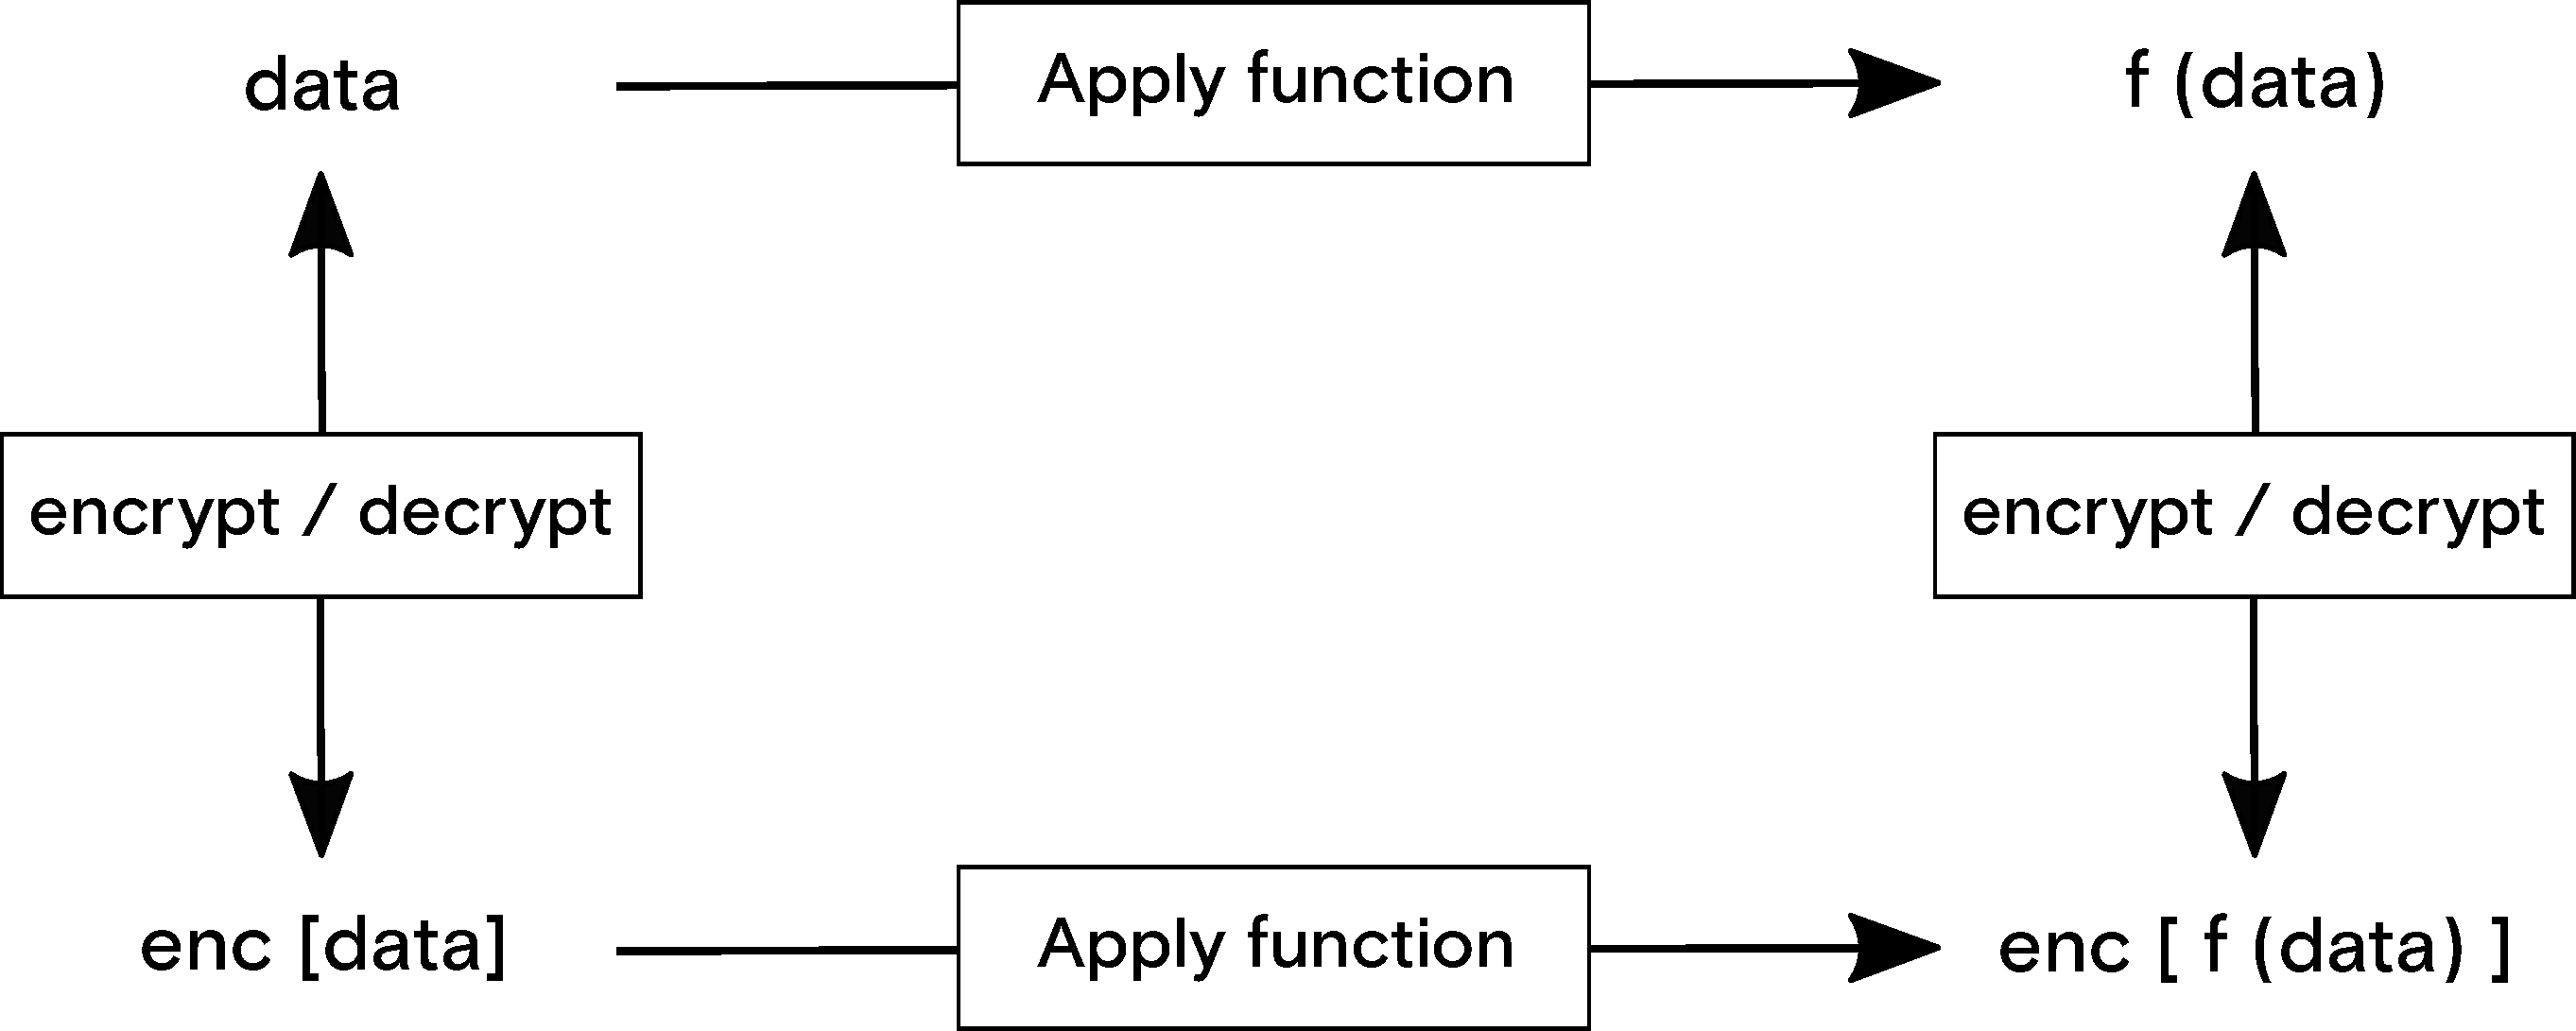
\includegraphics[height=5cm]{pdf/fhe.pdf}
      \end{figure}
    \end{frame}
\end{document}


